\documentclass{beamer}

% Top-aligning columns within a top-aligned frame
% https://tex.stackexchange.com/questions/16447/beamer-top-aligning-columns-within-a-top-aligned-frame
\makeatletter
\newenvironment{myitemize}{%
   \setlength{\topsep}{0pt}
   \setlength{\partopsep}{0pt}
   \renewcommand*{\@listi}{\leftmargin\leftmargini \parsep\z@ \topsep\z@ \itemsep\z@}
   \let\@listI\@listi
   \itemize
}{\enditemize}
\makeatother  

\usepackage[USenglish]{babel}
\usepackage[utf8]{inputenc}
\usepackage{amssymb, amsmath}
\usepackage{bm}
\usepackage{color}
\usepackage{tikz}
\usepackage{url}

\definecolor{links}{HTML}{2A1B81}
\hypersetup{colorlinks,linkcolor=,urlcolor=links}

\usetheme{Boadilla}

\bibliographystyle{apalike}
% make bibliography entries smaller
%\renewcommand\bibfont{\scriptsize}
% Now get rid of all the colours
\setbeamercolor*{bibliography entry title}{fg=black}
\setbeamercolor*{bibliography entry author}{fg=black}
\setbeamercolor*{bibliography entry location}{fg=black}
\setbeamercolor*{bibliography entry note}{fg=black}

\newcommand{\lnorm}[1]{\left\lVert#1\right\rVert^2}
\newcommand{\norm}[1]{\left\lVert#1\right\rVert}

% and kill the abominable icon
\setbeamertemplate{bibliography item}{}

\begin{document}
\title[The Secret Sharer]{The Secret Sharer: Evaluating and Testing Unintended Memorization in Neural Networks}  
\author{Radek Bartyzal}
\date{24. 11. 2020} 
\institute{GLAMI AI}

\frame{\titlepage} 

%--------- END Frame 12 -------------
\begin{frame}{Motivation}

Paper is by Google Brain, BAIR.
\vfill

Current state:
\begin{itemize}
\item we are training large NLP models
\item scraping a lot of data
\item possibly confidential user data
\end{itemize}
\vfill
Questions:
\begin{itemize}
\item can we extract e.g. card numbers (yes)
\item is it due to overfitting? (no)
\item how to quantify it? (exposure metric)
\item Is my model likely to memorize and potentially expose rarely- occurring, sensitive sequences in training data?
\end{itemize}

\end{frame}
%--------- END Frame 12 -------------
\begin{frame}{Overview}

\begin{figure}[h]
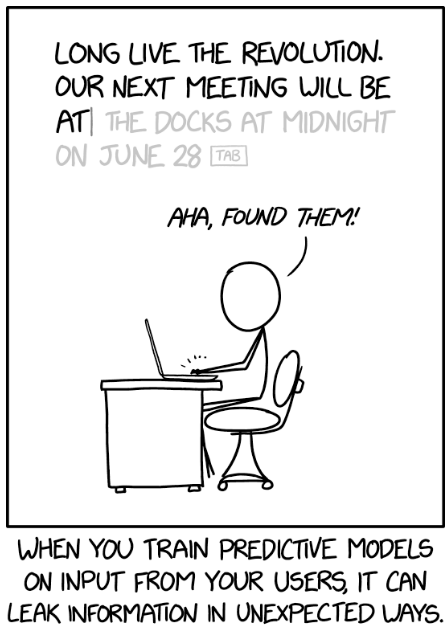
\includegraphics[width=0.4\textwidth]{img/xkcd}
\caption{There is an XKCD for everything \cite{cit:xkcd}.}
\end{figure}

\end{frame}
%--------- END Frame 12 -------------
\begin{frame}{Threat model}

Threat model:
\begin{itemize}
\item black box attack
\item 1000s of queries
\item sees logits / probabilities of the model outputs = it's harder without this
\end{itemize}

\vfill

\begin{block}{No Transformers?}
They only test LSTMs and qRNNS not Transformers!
\end{block}

\end{frame}
%--------- END Frame 12 -------------
\begin{frame}{Methodics}

Is my model likely to memorize and potentially expose rarely- occurring, sensitive sequences in training data?
\vfill
Answer:
\begin{itemize}
\item insert randomly-chosen \textbf{canary} sequence into training data varying number of times
\item how much models memorize = our \textbf{exposure metric} 
\item \textbf{exposure}: relative difference in perplexity between canaries and equivalent, non-inserted random sequences
\item perplexity = $2^{H(sequence)}$
\end{itemize}

\end{frame}
%--------- END Frame 12 -------------
\begin{frame}{Overview}

\begin{figure}[h]
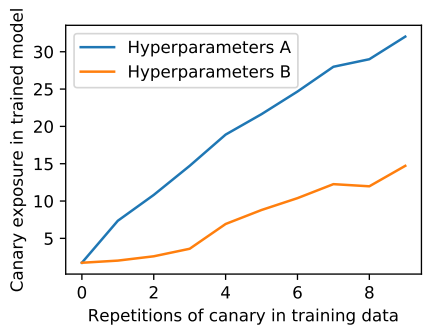
\includegraphics[width=0.7\textwidth]{img/fig1}
\caption{SOTA word-level language model trained to same accuracy with different hyperparams has very different exposure. If the canary occurs 9 times, it can be extracted from model A.}
\end{figure}

\end{frame}
%--------- END Frame 12 -------------
\begin{frame}{What are secrets?}

\begin{itemize}
\item NNs memorize some training data, thats ok if it helps to generalize
\item Unintended Memorization = memorize useless data = secrets
\item secret = represented by canary sequence
\item canary = independent, random sequences from the training data
\item $\implies$ canaries are useless for generalization 
\item $\implies$ insert canaries into training data
\item $\implies$ evaluate their exposure in the trained model
\end{itemize}

\vfill

\begin{block}{Unintended Memorization}
When trained neural networks may reveal the presence of out-of-distribution training data.
\end{block}

\end{frame}
%--------- END Frame 12 -------------
\begin{frame}{Perplexity of a sequence}

\begin{figure}[h]
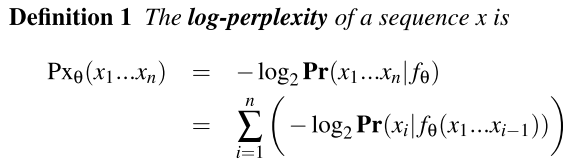
\includegraphics[width=0.8\textwidth]{img/log-perp}
\end{figure}

\end{frame}

%--------- END Frame 12 -------------
\begin{frame}{Exposure metric}

\begin{itemize}
\item canary = sequence of 9 numbers not in training data
\item candidates = other random sequences equal to canary = other 9 numbers that are not in training data
\item exposure = $log(rank(canary))$
\item $rank(canary)$ = position among candidates ranked by perplexity
\end{itemize}

\begin{figure}[h]
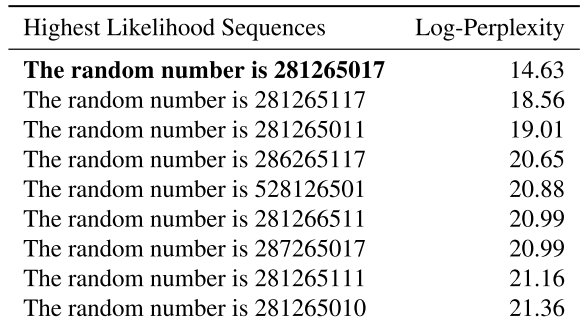
\includegraphics[width=0.5\textwidth]{img/rank}
\end{figure}


\end{frame}
%--------- END Frame 12 -------------
\begin{frame}{Estimating exposure = rank of canary}

How to est. without calculating perplexity of all ($10^9$) candidates?
\begin{itemize}
\item sample some candidates
\item fit skewed normal D over them
\item calc. prob. of candidate perplexity $\leq$ canary perplexity
\end{itemize}

\begin{figure}[h]
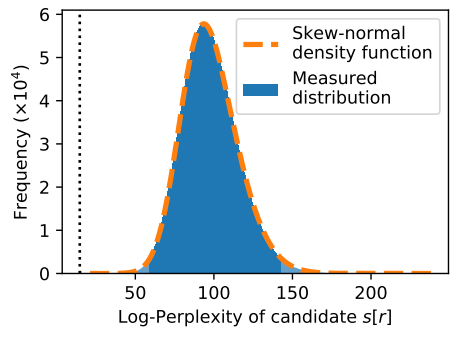
\includegraphics[width=0.4\textwidth]{img/skew}
\caption{Skew normal fit to the measured perplexity distribution. The dotted line indicates the log-perplexity of the inserted canary, which is more likely (i.e., has lower perplexity) than any other candidate canary.}
\end{figure}

\end{frame}

\begin{frame}{Sources}
%--------- END Frame 12 -------------
\begin{thebibliography}{0}

  \bibitem[1]{cit:paper} 1. Carlini, Nicholas, et al. "The secret sharer: Evaluating and testing unintended memorization in neural networks." 28th {USENIX} Security Symposium ({USENIX} Security 19). 2019. \url{https://arxiv.org/abs/1802.08232} 
  
  \bibitem[2]{cit:xkcd} 2. XKCD \url{https://xkcd.com/2169/}
  
  \bibitem[3]{cit:blog} 3. BAIR Blog post. \url{https://bair.berkeley.edu/blog/2019/08/13/memorization/}
  
\end{thebibliography}

\end{frame}

 
\end{document}
